\chapter{Background}
\label{Chapt2}
\section{Introduction}

This chapter will explore the fundamental information relevant to this project, with an emphasis on the world of DNS abuse and transparency. It will include a thorough investigation of the domain name system (DNS), its crucial function in the online community, and the variety of abuses it faces. The history of widely used policies and organisations aimed at stopping DNS abuse, including a thorough examination of the DNS Abuse Institute and its achievements, is essential to our investigation. A 'competition landscape' providing a critical examination of current market choices, from automated solutions to human tactics, will be provided as we navigate through the current methodology and technology deployed to detect and combat DNS abuse.  This analysis will also cover new developments that aim to improve DNS security and privacy, providing information on the use and consequences of technologies such as DNS over TLS (DoT) and DNS over HTTPS (DoH). The reader will obtain an in-depth understanding of the current situation of DNS abuse and the need for a more open, strong, and proactive strategy by analysing these various techniques and appreciating their strengths and weaknesses. This chapter emphasises the importance of the suggested solution in an era where digital authenticity is crucial, not only by providing information but also by laying the groundwork for its presentation as a better and essential progression in the battle against DNS abuse.

\section{Understanding DNS and Its Vulnerabilities}

The Domain Name System (DNS) is a crucial part of the infrastructure of the Internet, serving as the key that converts computer-understandable IP addresses into human-friendly domain names. Although the DNS plays a vital role in maintaining ongoing online activities, privacy and security problems still arise. The ScienceDirect paper "Domain Name System Security and Privacy: A Contemporary Survey" provides a thorough analysis of these concerns. This survey highlights the fundamental significance of the DNS while illuminating the weaknesses that malicious actors may take advantage of \cite*{sciencedirect2023dns}.

A variety of security threats exist, ranging from DNS infrastructure-targeting distributed denial of service (DDoS) assaults to cache poisoning and hijacking. Each of these attacks has the potential to do significant harm, including interruptions in service and the promotion of theft and spying. Due to the standard DNS design's lack of encryption, users' query data is vulnerable to abuse and eavesdropping, raising serious privacy problems. However, weaknesses do not mark the end of the story. In the same survey, new approaches are examined to improve DNS security and privacy. The use of DNSSEC (DNS Security Extensions), which authenticates DNS data and guarantees its integrity while repelling some types of attack, is one example of these advances in cryptographic security measures. Moreover, privacy-enhancing technologies are being used to encrypt DNS queries, preventing eavesdropping and manipulation, such as DNS over HTTPS (DoH) and DNS over TLS (DoT).

The environment of DNS threats and defences is always changing in sync with the internet. For systems to be robust and resilient, it is essential to understand these weaknesses and the continuous efforts being made to mitigate them. An in-depth discussion of DNS vulnerability details, the effects of these safety concerns, and creative solutions that aim to bring in a new era of DNS security and privacy will be provided in this section \cite{sciencedirect2023dns}.

\section{Current efforts and organisations combatting DNS Abuse}

Addressing DNS abuse is a complex challenge that requires coordinated efforts across various sectors of the Internet ecosystem. Foremost among the entities dedicated to this cause is the DNS Abuse Institute. Established with a focused mission, the DNS Abuse Institute aims to combat DNS abuse and ensure the safety and security of the domain name system. Their goal is to assist the internet community in identifying, reporting, and mitigating instances of DNS abuse, thereby fostering a safer online environment \cite{dnsabuseinstitute2023}. The Institute emphasises the development and support of initiatives that improve understanding and mitigation of DNS abuse. They introduce innovative solutions like the "Compass Dashboards," which provide essential data and insights to registries and registrars, aiding them in making informed decisions to combat abuse. Furthermore, the DNS Abuse Institute is committed to transparency and education. They regularly publish reports and bulletins, such as the "DNSAI 2022 Annual Report" and the "DNSAI Bulletin 2023 04; Account Takeovers," offering a detailed view of the state of DNS abuse and the steps taken to address it \cite{dnsabuseinstitute2023} . These publications serve as a valuable resource for stakeholders looking to understand the landscape of DNS abuse and the collective efforts to mitigate it \cite{dnsai2022report}.

In addition to the DNS Abuse Institute, organisations like the Internet Corporation for Assigned Names and Numbers (ICANN) play a critical role in the global effort to monitor and reduce DNS abuse. ICANN's reports and initiatives provide insights and guidelines that shape policies and practices in the domain name industry. Their work involves collaboration with various stakeholders, including registries, registrars, and policy-making bodies, to develop and enforce standards that minimize DNS abuse while maintaining the openness and interoperability of the internet \cite{icann2022dnsabuse} . These organizations, along with numerous others involved in the fight against DNS abuse, contribute to a multi-faceted approach that includes policy development, technological innovation, and community engagement.\cite{dnsabuseinstitute2023} By highlighting the objectives, methods, and reports published by these entities  \cite{dnsai2022report}   , this section will provide a comprehensive view of the current efforts and organizations dedicated to combating DNS abuse, illustrating the collaborative nature of this ongoing battle \cite{icann2022dnsabuse} .

\section{DNS Privacy and Security Enhancements}

The digital world is changing, and so too is the need for enhanced privacy and security measures within the Domain Name System (DNS). Significant advancements have been made to protect users and their data, particularly through the implementation of DNS over TLS (DoT) and DNS over HTTPS (DoH). These technologies represent a paradigm shift in DNS query encryption, aiming to address privacy concerns and secure communication between clients and servers. DNS over TLS (DoT) offers a way to encrypt DNS requests and answers, making it harder for bad actors to simply intercept or change the data. This technology is essential to protect user privacy and stop man-in-the-middle and eavesdropping attacks. In the same way, DNS over HTTPS (DoH) leverages the security features and broad acceptance of HTTPS to protect DNS requests within the HTTPS protocol, adding an extra degree of protection.

The paper "DNS Privacy in Practice and Preparation," which focusses on how these technologies are being accepted and put into effect, provides an in-depth review of these developments. It emphasises how important DoT and DoH are to protecting DNS privacy and how key public DNS service providers are supporting these more and more. The implementation of DoT and DoH is not without difficulties, regardless of their advantages. Their effectiveness depends on factors like performance concerns and the requirement for extensive implementation across multiple platforms. The study also highlights how critical TCP Fast Open (TFO) is to reducing TCP-based DNS query latency, which is essential to balance privacy and speed  \cite{acm2023dnsprivacy}  .

\section{Different Forms of DNS Abuse}

DNS abuse takes many forms, each with its procedures and effects on users and the internet as a whole. It is essential to understand these various pieces of evidence to create responses and regulations that work. This section will examine the comprehensive analysis of DNS abuse as presented, going into the description, mechanism, and impact of each kind.

\subsection{Phishing}
\begin{itemize}
    \item \textbf{Description:} Phishing is a technique aimed at deceiving individuals by creating website addresses that mimic those of companies, to trick users into revealing sensitive information such as login credentials, credit card numbers, or personal identification information.\cite{webinarcare2023dnsstats}
    \item \textbf{Mechanism:} This deception often occurs through emails or messaging services that direct users to websites resembling authentic ones.\cite{jakobsson2006phishing}
    \item \textbf{Impact:} Victims may suffer identity theft, financial fraud, and security compromise.
\end{itemize}

\subsection{Confusable Domains (Typosquatting)}
\begin{itemize}
    \item \textbf{Description:} Registering domain names that look visually similar to popular websites, taking advantage of typing errors or character similarities.\cite{inta2023dnstypo}
    \item \textbf{Mechanism:} Users may accidentally visit these websites when making a typo in a URL, potentially exposing them to malware or phishing attempts.
    \item \textbf{Impact:} Deception of users and potential harm to brand reputation.\cite{edelman2008typosquatting}
\end{itemize}

\subsection{Domain Hijacking}
\begin{itemize}
    \item \textbf{Description:} Unauthorized acquisition of domain names by exploiting security vulnerabilities in the domain registration system.\cite{inta2023dnstypo}
    \item \textbf{Mechanism:} Attackers may use tactics like social engineering, phishing, or exploiting security loopholes to gain control over a domain.
    \item \textbf{Impact:} Loss of website control, redirection to malicious sites, and potential data breaches.
\end{itemize}

\subsection{Botnets}
\begin{itemize}
    \item \textbf{Description:} Botnets involve controlling a group of computers infected with malware, used to carry out attacks or spread spam and malware.\cite{citpyour}
    \item \textbf{Mechanism:} Malware infects unsuspecting users’ computers, incorporating them into a network under the attacker's control.
    \item \textbf{Impact:} Can result in large-scale DDoS attacks, mass spam campaigns, and widespread malware dissemination.
\end{itemize}

\subsection{Fast Flux Hosting}
\begin{itemize}
    \item \textbf{Description:} A technique used to conceal the location of websites associated with phishing and malware distribution.\cite{lin2013genetic}
    \item \textbf{Mechanism:} Involves a network of compromised hosts that regularly modify DNS records to evade detection.
    \item \textbf{Impact:} Makes tracking and shutting down malicious sites difficult.
\end{itemize}

\subsection{Domain Generation Algorithms (DGA)}
\begin{itemize}
    \item \textbf{Description:} DGAs generate domain names that act as meeting points for botnets.\cite{antonakakis2012throw}
    \item \textbf{Mechanism:} Malicious software uses algorithms to generate a sequence of domain names for command-and-control servers.
    \item \textbf{Impact:} Adds complexity to efforts to disrupt botnet command and control channels.
\end{itemize}
\captionsetup{font= small}
\begin{figure}[ht!]
\centering
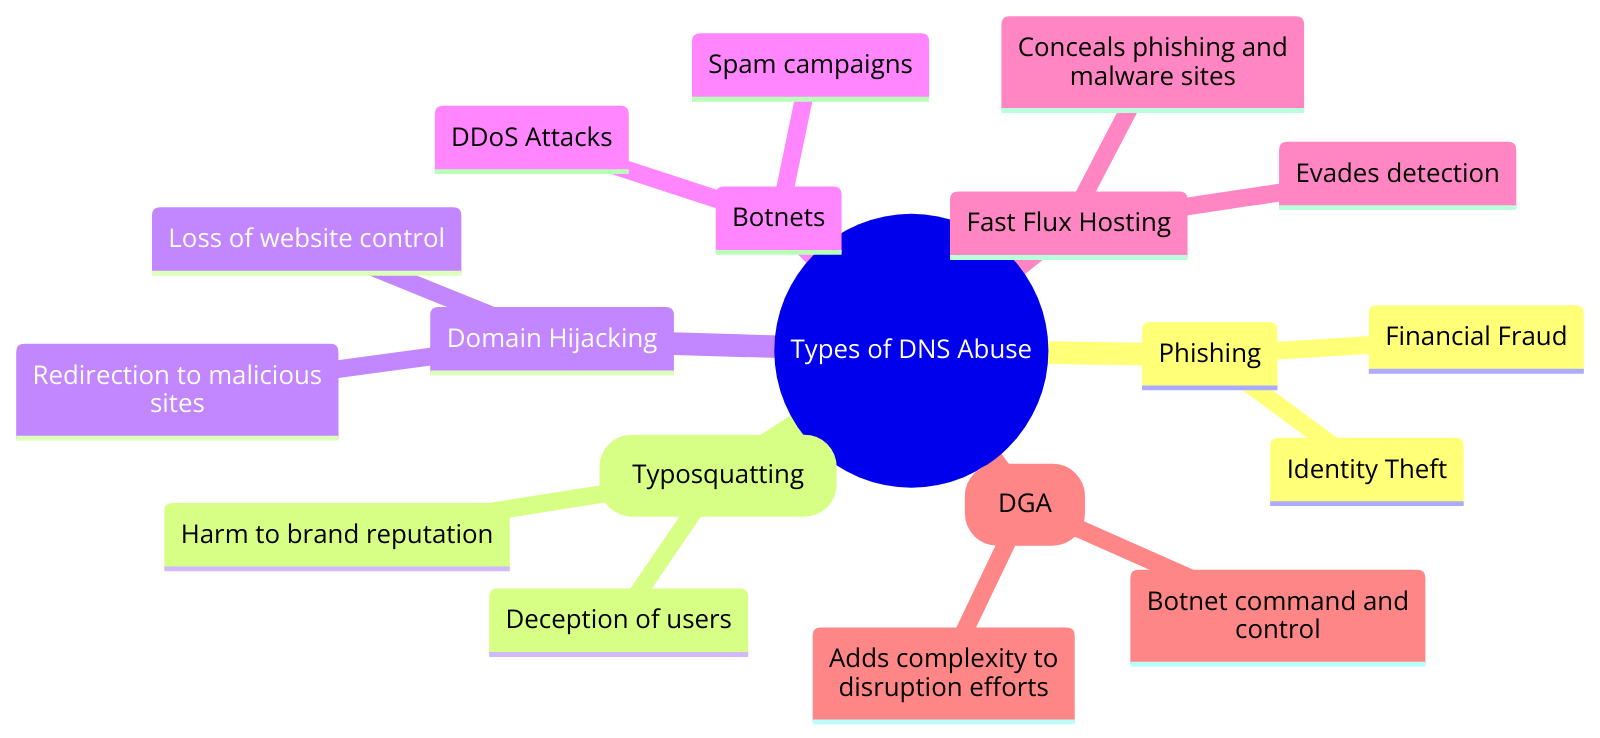
\includegraphics[width=1.0\textwidth]{background/DNSabuseForms.png}
\caption{Impact of DNS Abuse}
\label{fig:figureThree}
\end{figure}



\section{How DNS Abuse Harms Users}

DNS abuse has serious and detrimental effects for both users and organisations, going beyond basic technological disruptions. Identity theft is among the most direct and direct effects. Phishing attacks, a frequent type of DNS abuse, use realistic websites to trick visitors into revealing sensitive data. Such attacks can produce information that results in financial theft, unauthorised access to accounts, and long-term damage to a person's reputation and credit.

\subsection{Identity Theft}
\begin{itemize}
    \item \textbf{Phishing:} Phishing attacks often use domain names that imitate legitimate websites, fooling users into providing sensitive information such as usernames, passwords, or financial details, leading to potential identity theft.\cite{godaddy2023dnsabuse, jakobsson2006phishing}
\end{itemize}

\subsection{Financial Loss}
\begin{itemize}
    \item \textbf{Deceptive Transactions:} Users may be tricked into making payments to deceptive websites or unknowingly disclose their credit card information, resulting in financial losses.\cite{godaddy2023dnsabuse, bohme2013economics}
\end{itemize}

\subsection{Data Breach}
\begin{itemize}
    \item \textbf{Malware:} Malicious software spread through compromised DNS systems can allow unauthorized access to corporate data, leading to data breaches.\cite{icann2022dnsabusetrends, fowler2016data}
\end{itemize}

\subsection{System Compromise}
\begin{itemize}
    \item \textbf{Malware Infection:} Systems infected with malware due to DNS abuse can be exploited for further attacks, including the creation of botnets or the distribution of ransomware, resulting in system compromise.\cite{dotmagazine2022dnsabuse, saxe2018malware}
\end{itemize}
\captionsetup{font= small}
\begin{figure}[ht!]
\centering
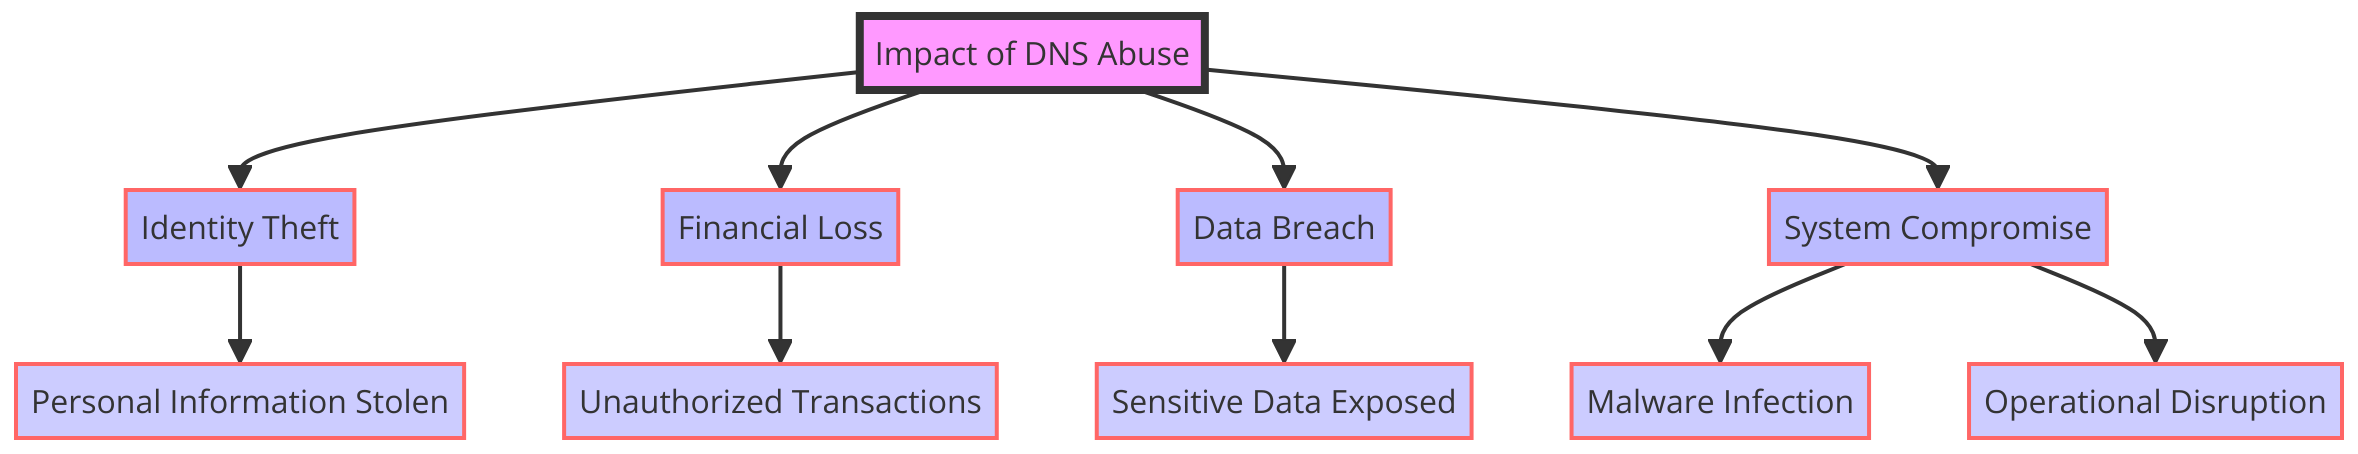
\includegraphics[width=1.0\textwidth]{background/DNSabuseHarm.png}
\caption{Different Forms of DNS Abuse}
\label{fig:figureFour}
\end{figure}


\section{Future Dangers of DNS Abuse}

As technology develops, so do cyber attackers' strategies and tools, creating a dynamic environment for DNS abuse that could present new risks in the future. The sophistication of attacks has increased, which is a major issue. Cybercriminals are always creating increasingly sophisticated methods to take advantage of DNS, such as creating more convincing phishing schemes and using complex virus distribution networks.

\subsection{Increased Sophistication}
\begin{itemize}
    \item \textbf{Evolving Techniques:} Cyber attackers are constantly developing more sophisticated techniques to exploit DNS, such as advanced phishing schemes and malware distribution.\cite{icann2022dnsabusetrends, wrightson2014advanced}
\end{itemize}

\subsection{IoT Vulnerabilities}
\begin{itemize}
    \item \textbf{Expanding Vulnerabilities:} The widespread adoption of Internet of Things (IoT) devices, which often lack robust security measures, presents a growing target for DNS-based attacks.\cite{circleid2020dnstrends, mahmoud2015internet}
\end{itemize}

\subsection{Infrastructure Attacks}
\begin{itemize}
    \item \textbf{DNS as a Prime Target:} Attacks on DNS infrastructure can disrupt internet services on a large scale, including DDoS attacks targeting DNS providers or exploiting weaknesses in DNS protocols.\cite{dotmagazine2022dnsabuse, dooley2017dns}
\end{itemize}

\subsection{Deepfakes and AI}
\begin{itemize}
    \item \textbf{AI-Enhanced Phishing:} The use of AI technologies, such as deepfakes, has made phishing attacks more convincing and deceptive, manipulating audio and video content to impersonate trusted entities.\cite{icann2022dnsabusetrends, schick2020deep}
\end{itemize}

\subsection{Cloud Computing Vulnerabilities}
\begin{itemize}
    \item \textbf{Targeting Cloud Services:} As organizations increasingly rely on cloud-based services, cybercriminals are exploiting DNS vulnerabilities to attack these platforms, potentially leading to data breaches and service disruptions.\cite{mather2009cloud}
\end{itemize}

\subsection{Mobile Device Exploitation}
\begin{itemize}
    \item \textbf{Mobile DNS Attacks:} The rising usage of mobile devices has led cybercriminals to target smartphones and tablets through DNS-based attacks, which can lead to data theft and the spread of malware.\cite{au2016mobile}
\end{itemize}

\subsection{Cryptocurrency and Blockchain Exploitation}
\begin{itemize}
    \item \textbf{Crypto-Related DNS Attacks:} Attackers could exploit DNS vulnerabilities to redirect users to fake cryptocurrency exchanges or blockchain platforms, leading to financial fraud and theft of digital assets.\cite{bashir2019advanced}
\end{itemize}

\subsection{Political and Information Warfare}
\begin{itemize}
    \item \textbf{DNS in Cyber Warfare:} The manipulation of domain name systems can be used to spread misinformation or disrupt services during significant political events, serving as a tool for political and information warfare.\cite{chapple2021cyberwarfare}
\end{itemize}

\subsection{Exploiting Emerging Technologies}
\begin{itemize}
    \item \textbf{Abuse in New Tech Domains:} As new technologies such as 5G, AI, and quantum computing advance, tactics involving DNS abuse are likely to evolve, potentially leading to more sophisticated attacks.\cite{brunner2021cybersecurity}
\end{itemize}

\subsection{Supply Chain Attacks}
\begin{itemize}
    \item \textbf{DNS in Supply Chain Compromise:} DNS manipulation can also be employed as part of supply chain attacks, targeting software updates or cloud-based services to compromise organizations.\cite{boyson2014cyber}
\end{itemize}

By understanding these future dangers and emerging trends, stakeholders can better prepare and adapt their strategies to anticipate and counteract the evolving nature of DNS abuse.

\clearpage
\captionsetup{font= small}
\begin{figure}[ht!]
\centering
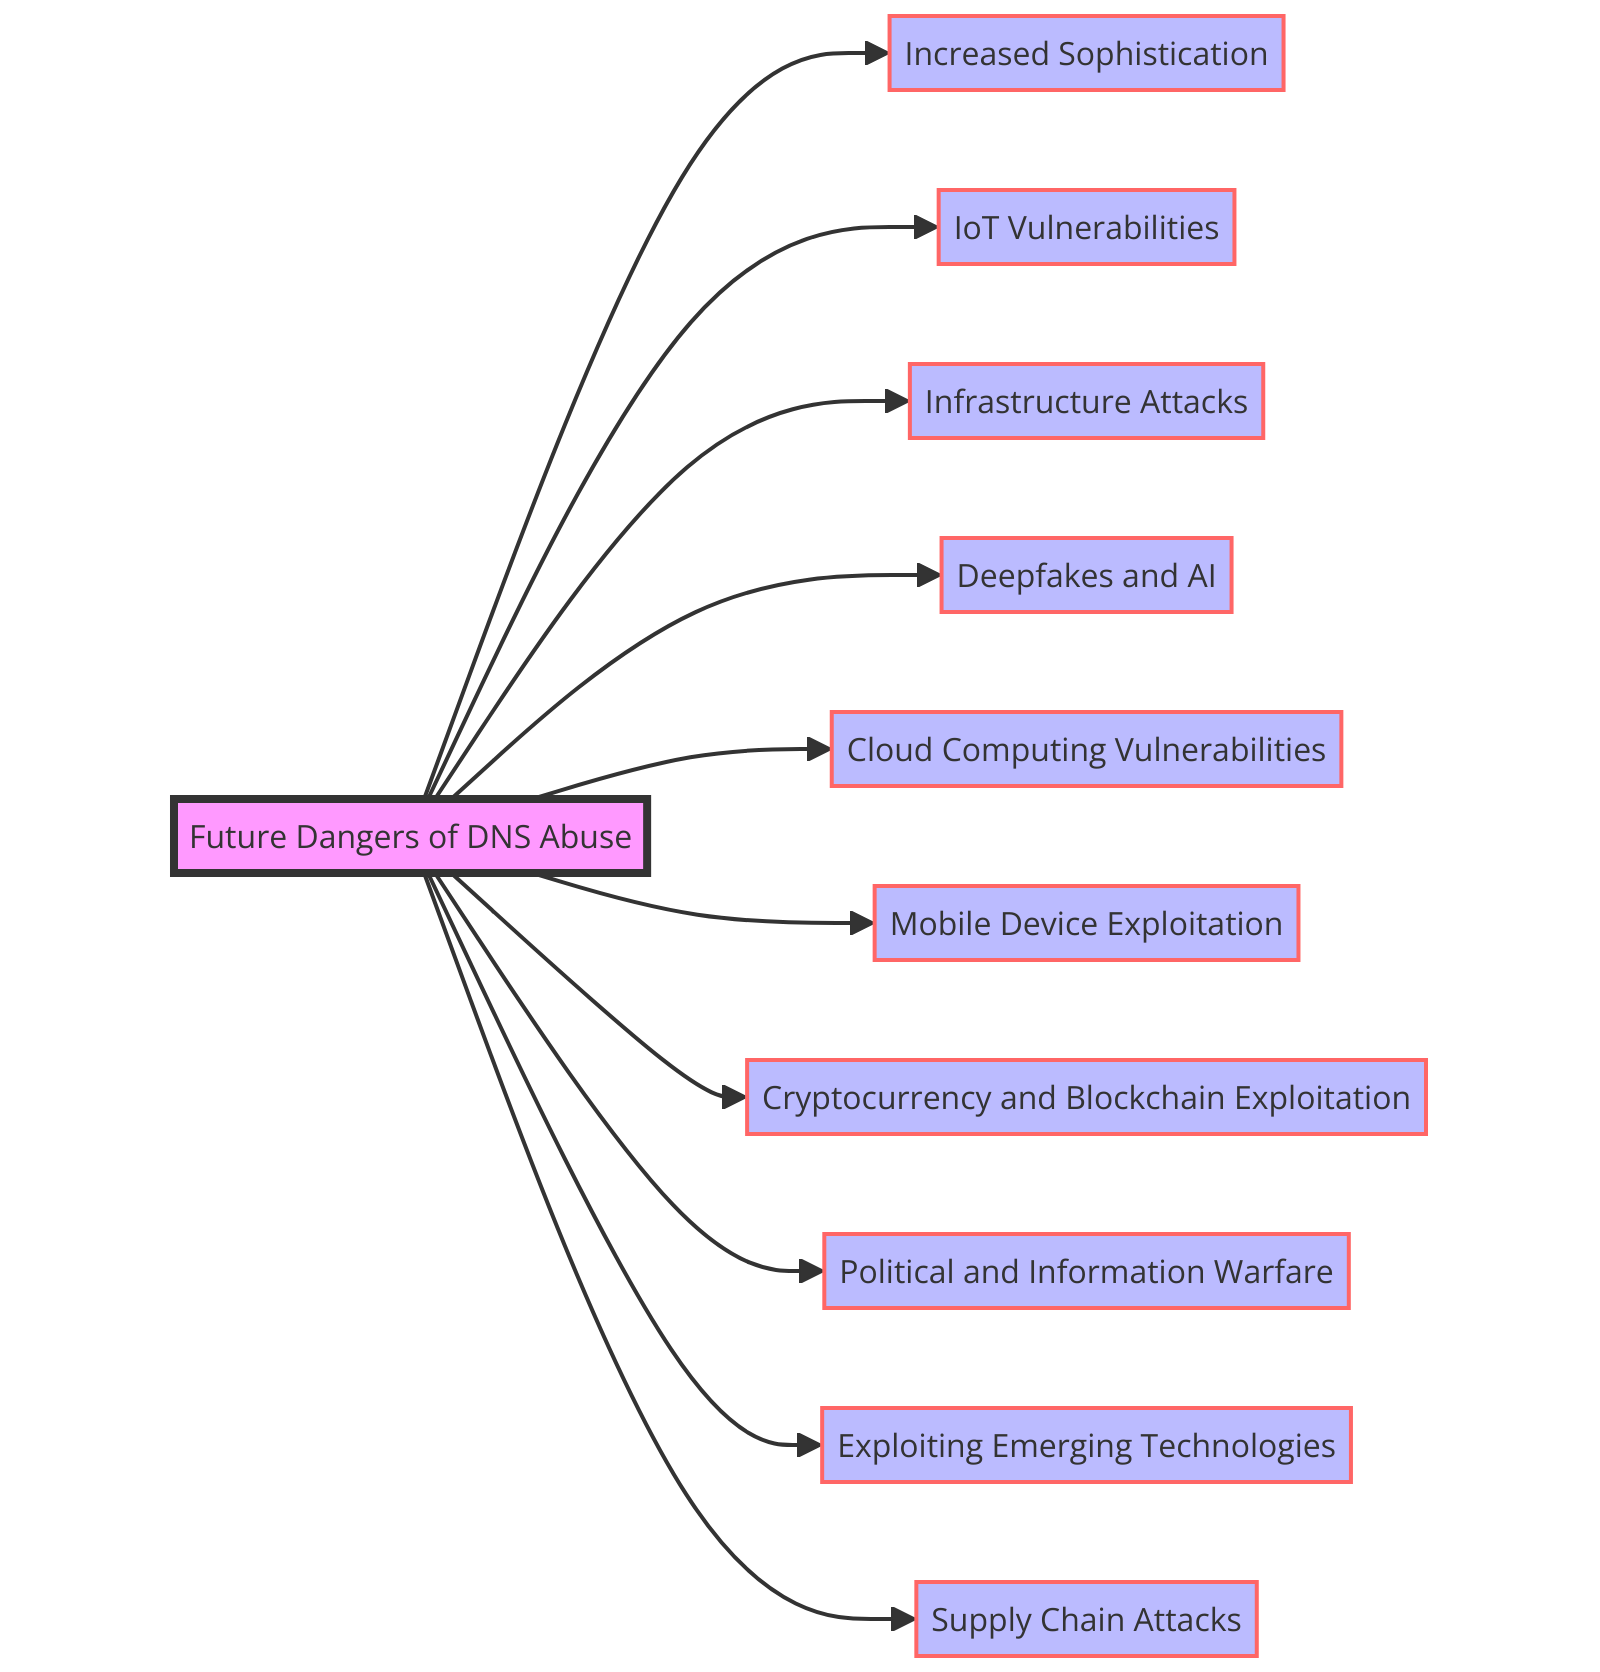
\includegraphics[width=1.2\textwidth]{background/DNSfutureDanger.png}
\caption{Future dangers of DNS abuse}
\label{fig:figureFive}
\end{figure}
\clearpage

\section{Mitigation Strategies and Best Practices }

To address the broad nature of the threats, combating DNS abuse requires an integrated strategy that integrates multiple strategies and best practices. Setting up procedures for reporting and monitoring is one fundamental tactic. Automated systems have the ability to track domain name registration patterns that may indicate DNS abuse, and protocols for reporting questionable actions can help ensure prompt intervention \cite{icannndnssec}. To confirm security and ensure that systems have not been compromised, regular audits of DNS setups and domain registrations are also necessary \cite{lucas2021tls} .

\begin{enumerate}
    \item \textbf{Monitoring and Reporting}
    \begin{itemize}
        \item Implementation: Use automated systems to monitor the registration of domain names for patterns that may indicate DNS abuse \cite{icannndnssec}. Establish procedures for reporting activities to authorities or cybersecurity organisations \cite{lucas2021tls}.
    \end{itemize}
    \item \textbf{Security Awareness Training}
    \begin{itemize}
        \item Implementation: Develop training programs for users and IT staff with a focus on recognizing phishing attempts, practicing browsing habits, and understanding DNS security.
    \end{itemize}
    \item \textbf{DNS Security Extensions (DNSSEC)}
    \begin{itemize}
        \item Implementation: Deploy DNSSEC to ensure the integrity of DNS data. This involves signing DNS records to protect against modifications and DNS spoofing.
    \end{itemize}
    \item \textbf{Multi-Factor Authentication (MFA)}
    \begin{itemize}
        \item Implementation: Enforce multifactor authentication (MFA) for domain registrars and interfaces used to manage DNS \cite{icannndnssec}. This adds a layer of security beyond passwords, helping to prevent unauthorised domain transfers or alterations \cite{moghaddam2014ecco}.
    \end{itemize}
    \item \textbf{Blacklisting and Takedown Services}
    \begin{itemize}
        \item Implementation: Collaborate with cybersecurity firms to identify and blacklist domains engaged in malicious activities. Establish response teams dedicated to taking down domains involved in DNS abuse.
    \end{itemize}
    \item \textbf{Collaboration}
    \begin{itemize}
        \item Implementation: Foster collaboration among internet service providers (ISPs), domain registrars, governments, and cybersecurity organizations. Share intelligence and best practices to collectively enhance defense against DNS abuse \cite{skopik2017collaborative}.
    \end{itemize}
    \item \textbf{Regular Audits}
    \begin{itemize}
        \item Implementation: Conduct security audits of domain registrations and DNS configurations to verify their security and ensure they have not been compromised \cite{coronado2014auditing}.
    \end{itemize}
    \item \textbf{Machine Learning}
    \begin{itemize}
        \item Implementation: Using AI and machine learning algorithms to analyse patterns in DNS traffic and proactively predict instances of DNS abuse \cite{icannndnssec}. This proactive approach enables the identification of threats before they materialise \cite{tsukerman2019machine}.
    \end{itemize}
    \item \textbf{Geo-Blocking and IP Filtering}
    \begin{itemize}
        \item Implementation: Deploy geo-blocking and IP filtering techniques to limit access to DNS services from regions that have a history of DNS abuse. This can reduce the risk that attackers will use these services to carry out malicious activities or distribute malware \cite{meeseedited}.
    \end{itemize}
    \item \textbf{Enhanced Domain Validation Procedures}
    \begin{itemize}
        \item Implementation: Enhance the domain registration process by implementing validation procedures. This may involve verifying the identity of individuals or organizations that register domains, especially domains that resemble brands or fall into sensitive categories. By taking these measures, we can strengthen security and mitigate risks associated with fraudulent domain registrations.
    \end{itemize}
\end{enumerate}

Each of these strategies plays a crucial role in creating a comprehensive defence against DNS abuse. By integrating these tactics, organisations can establish robust, proactive measures to detect, prevent, and mitigate the ever-evolving threats posed by DNS abuse.
\captionsetup{font= small}
\begin{figure}[ht!]
\centering
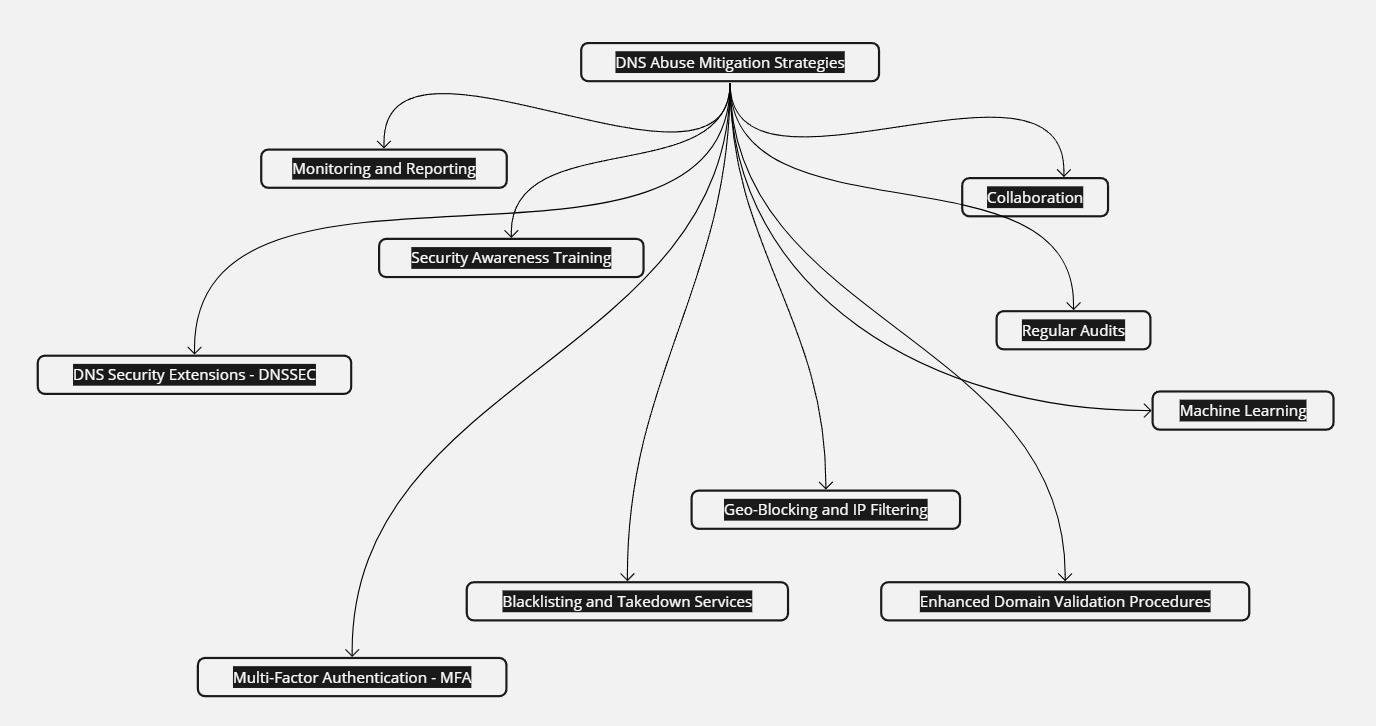
\includegraphics[width=0.8\textwidth]{background/DNSabuseMiti.jpg}
\caption{Future dangers of DNS abuse}
\label{fig:figureSix}
\end{figure}

\section{Summary and Synthesis}

This chapter has examined all aspects of DNS abuse,  the various forms, the serious harm it does, as well as potential future threats and new trends. To create efficient regulations and countermeasures, it is essential to understand the extent and consequences of DNS abuse. The conversation emphasised DNS's vital function in the digital ecosystem as well as its susceptibility to abuse.Significant progress towards resolving these issues has been made by organisations like the DNS Abuse Institute and ICANN, as well as developments in DNS privacy and security technologies like DoT and DoH. However, as new technologies are incorporated into the equation and the threat environment changes in sophistication, it becomes increasingly important to adopt alert, flexible and cooperative strategies.  

The mitigation techniques and best practices discussed in this chapter provide a roadmap for mitigating DNS abuse. Every tactic contributes to a defence mechanism, from advanced technology solutions and improved methods for validation to monitoring and reporting. It is impossible to overestimate the value of cooperation, regular checks, and the application of cutting-edge technologies to anticipate and stop DNS abuse. After analysing the data, it is evident that a team effort is needed to comprehend, track, and mitigate DNS abuse. A complex strategy that integrates multiple techniques and encourages collaboration across industries is required instead of a single, insufficient strategy. Our approaches to preserving the integrity and security of the DNS and, consequently, the larger internet infrastructure must adapt as does the digital environment.

By understanding the connections between different aspects of DNS abuse and reinforcing the collective effort required for effective mitigation, stakeholders can be better prepared to face the challenges ahead. This chapter sets the stage for further research and action, with the aim of contributing to a safer and more secure digital world.

\chapter{State of the Art}

This chapter explores the strategies being employed to mitigate DNS abuse as well as new developments in this field. Explores and evaluates the effectiveness and transparency of multiple mitigation techniques, including DNS filtering and threat intelligence in which information about cyber attacks that experts organise and analyse. Additionally, the use of domain-generating techniques and DoT and DoH are two novel forms of DNS abuse that are highlighted in this section. Along with the role of AI and machine learning in identifying and mitigating DNS abuse is covered. The final half of the section includes a discussion on potential future research areas and technologies to improve DNS abuse mitigation. Case studies offer practical insights into DNS abuse occurrences. 

\section{Current Strategies and Their Effectiveness in Relation to DNS Abuse}

DNS abuse presents a significant challenge for internet entities involved in domain name management. Various approaches are employed to mitigate such abuse, including DNS filtering, which regulates access to specific websites and prevents you from accessing malicious sites that can administer phishing and ransomware. Additionally, threat intelligence methodologies leverage data analysis to identify potential risks, as exemplified by \cite{schmid2021thirty}. Anomaly detection plays a role in identifying suspicious DNS activities indicative of malicious intent using Packet Analysis to analyse individual packets for DNS allowing for real-time detection and statistical analysis, which involves performing statistical analysis on a large dataset of DNS traffic. However, these methods can encounter operational challenges, such as errors and the need for fast access to critical threat data. 

\subsection{Mitigation Strategies}

Different methods are employed to mitigate DNS abuse, including the implementation of tools for blocking, awareness of potential threats, and identification of anomalous behaviour. DNS filtering entails the regulation of website access based on predetermined rules, which can have varied outcomes depending on the context in which can happen in different environments such as register and registry in which it implements mechanisms to compare DNS names to the block list and given set of rules then take the necessary action such as homographs attacks in which DNS filtering mechanism play a role in mitigating them by comparing domain names against blocklists and predefined tule to identify potentially malicious homographs as stated earlier. Threat intelligence plays a role in identifying potential dangers and detecting unusual activities within the DNS, as noted \cite{rizvi2022application}, such as allowing the proactive identification and assessment of potential threats and malicious activities which includes detecting patterns indicative of phishing, domain hijacking, malware distribution, and other forms of DNS abuse. Evaluating the effectiveness of these methods requires careful consideration of their performance in real-world scenarios. For instance, while DNS filtering can effectively block malicious content, it may inadvertently permit harmful elements to bypass the filtering process, potentially impacting user experience. Similarly, the efficacy of threat intelligence relies on the timeliness and accuracy of the data utilized. However, identifying anomalous behaviour poses challenges, as distinguishing between malicious actions and legitimate activities performed in innovative ways can be challenging.

\subsection{Evaluation of Transparency}

Demonstrating the mechanisms through which DNS abuse can be mitigated is great step in fostering trust among stakeholders, including internet users, businesses, and policymakers. Simplified and transparent approaches to DNS abuse mitigation underscore a commitment to accountability and collaborative efforts in addressing abuse. Transparency in the context of the mitigation of DNS abuse includes clear communication of mitigation measures, disclosure of incidents, and access to information regarding decision-making processes. According to \cite{chaganti2023survey}, organisations that are forthcoming about their objectives tend to engage in regular updates and dialogue with the community, contributing to the clarity and integrity of the DNS.

\section{Emerging Trends in DNS Abuse}

Advancements in DNS abuse are altering the landscape of online security, introducing novel challenges and vulnerabilities. Among these emerging threats, sophisticated techniques such as the utilisation of DNS over TLS (DoT) and DNS over HTTPS (DoH) mechanisms have gained prominence. These protocols aim to enhance privacy and security by encrypting DNS queries, but simultaneously, they offer adversaries new avenues to obfuscate malicious traffic, complicating detection efforts. Furthermore, the proliferation of Domain Generation Algorithms (DGA) poses significant risks, as highlighted by \cite{kapoor2021ransomware}.  DGAs generate numerous seemingly random domain names, complicating the identification of potential threats. As the dynamics of the DNS infrastructure evolve, it is imperative for cybersecurity professionals to remain abreast of these developments. Continuous refinement of strategies and proactive measures is essential to counteract adaptive strategies employed in DNS abuse, thus safeguarding the integrity and trustworthiness of internet systems.

\subsection{New Forms of DNS Abuse}

The field of cybersecurity is rapidly advancing, bringing forth new challenges as it evolves, and constantly moving the goalposts for defence mechanisms. The introduction of DNS over TLS (DoT) and DNS over HTTPS (DoH) is akin to a double-edged sword. Although these encryption protocols were designed to enhance privacy and security by encrypting DNS queries, they inadvertently provide attackers with means to disguise malicious traffic. This broadens the attack surface, affecting everything from individual consumer devices to extensive corporate networks. For instance, attackers could leverage DoT and DoH in enterprise settings to circumvent outdated security controls and establish hidden communication channels. Moreover, Domain Generation Algorithms (DGAs) play a significant role in the cyber threat landscape by automatically generating a vast number of random domain names, making it extremely difficult to identify and shut down malicious sites. \cite{kaur2023artificial}. This tactic, integral to botnet command and control (C2) operations, significantly complicates the efforts of cybersecurity defences to predict and mitigate threats.
The adoption of DoT and DoH offers several benefits, such as enhanced privacy by preventing the surveillance of DNS queries and improved security through the encryption of DNS traffic, which hampers hackers' attempts to intercept or manipulate data. However, these protocols also enable attackers to conceal their malicious activities, which poses challenges for traditional DNS security systems in detecting and filtering harmful content. Furthermore, these protocols might inadvertently bypass content filtering policies, leading to potential security breaches within organisations.
Conversely, DGAs provide attackers with a method to evade detection and maintain C2 communications, as the dynamically generated domains are difficult to predict and pre-emptively block. This results in an overwhelming number of domain names for security mechanisms to monitor, complicating the threat intelligence process and necessitating continuous vigilance and blacklist updates. The widespread adoption of these technologies underscores the need for cybersecurity professionals to adopt a proactive and informed stance, understanding their potential for exploitation and developing comprehensive strategies. These strategies must strike a balance between the benefits of encryption and domain generation and the imperative to prevent DNS abuse, ensuring the integrity and security of the online environment.


\subsection{Predictive Measures and Their Transparency}

Efforts to mitigate DNS abuse are geared towards promptly halting such activities by utilizing complex systems and advanced machine learning algorithms to detect patterns indicative of abuse. Articulating and sharing insights about the decision-making processes in predictive modelling is deemed crucial as well as the efforts by registrars and registries, acting together, in the context of DNS Abuse Transparency are comprehensive. These entities will invoke a wide range of mitigation measures to minimise the damage and losses related to the DNS, which will ensure the development of a more secure and trusted Internet environment.Some key mitigation strategies are account-based remediation in the way that accounts which are maliciously generated are locked out and further validated, in addition to monitoring third-party feeds and reports from cybersecurity organisations, law enforcement, and the public to discover and address abuse early. Moreover, this mitigation entails malware analysis, which comes from attacks to the communication infrastructure and the corresponding IP addresses, through either suppression or sinkholing in the context of botnets and the use of Domain Generation Algorithms (DGAs) that direct botnet traffic. \cite{ M3AAWG2024} Most specifically, sinkholing is an authoritative measure that directs traffic from abusive domains to harmless servers and allows studies to take place on traffic sources and the extent of compromise. Compliance with legal and contractual requirements further underscores the actions of registrars and registries against DNS abuse, ensuring that their actions in mitigation are within the context of the ICANN agreements and local laws. The evidentiary evaluation of real-time black hole lists (RBLs), in addition to the responsible role of trusted notifiers, further increases the effectiveness and accuracy of mitigating actions, to filter and validate reports on abuse, so that proper responses may be made. This multi-pronged approach on the part of the registrars and the registries towards the mitigation of DNS abuse does not only emphasize the proactive and reactive measures but also the possibilities of increased transparency as far as reporting and publicizing the actions in place against DNS abuse are concerned. Such transparency is key to building trust, open for accountability, and creating an environment conducive to stakeholders' collaboration for the more effective fight against abuse in the DNS ecosystem. This transparency helps to understand the rationale behind the predictions, map the data used for model training, and clarify the methods that guide decision making, as highlighted in \cite{hussain2022software}. Striking a balance between the complexity of predictive models and their interpretability is a significant challenge. Therefore, it is essential to approach this challenge with caution, ensuring that the models are not only effective in identifying DNS abuse but also accessible for thorough examination and accountability.

\clearpage
\captionsetup{font= small}
\begin{figure}[ht!]
    \centering
    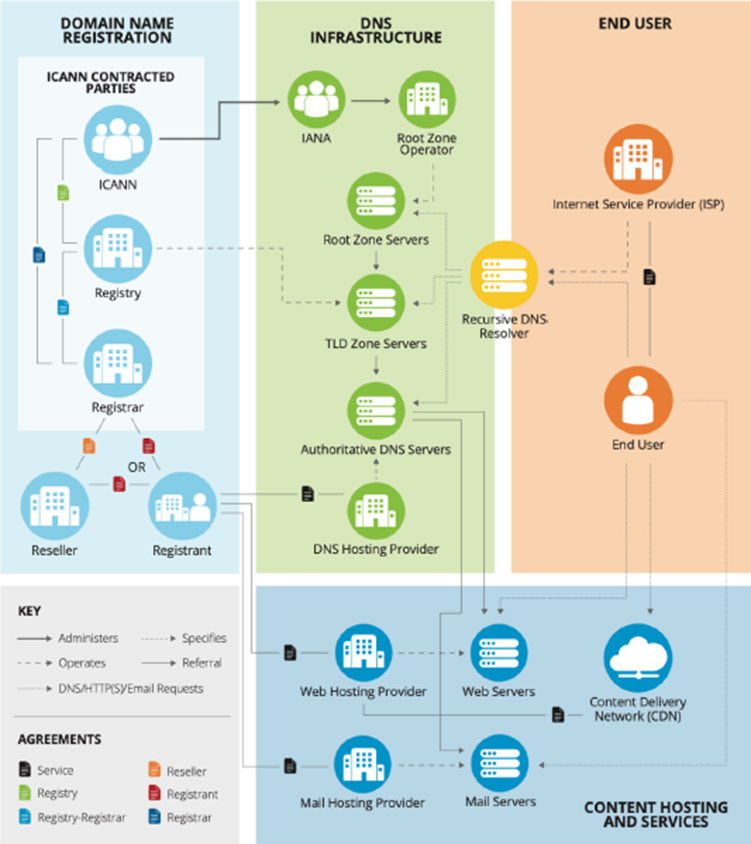
\includegraphics[width=1.0\linewidth]{background/DNSECO.png}
    \caption{Conceptual Diagram of the DNS Ecosystem Portion Contractually Related to ICANN (image
courtesy of Verisign and originally published in SSAC 115)}
    \label{fig:fig14}
\end{figure}
\clearpage

\section{Technological Advancements}

The mitigation of DNS abuse is increasingly influenced by the integration of artificial intelligence (AI) and machine learning technologies \cite{goethals2021enabling}. At the helm of this evolution are innovative tools like the iQ Domain Risk Score, which employs machine learning and string analytics to proactively detect potential domain abuses now of registration \cite{dnsabuseAI2023}. This tool aims to act as a preventive measure by analysing domains against criteria indicative of malicious intent, thereby attempting to stop abuse before it even starts. Additionally, the field is witnessing a transformative shift in analysing abuse report evidence through the adoption of Large Language Models (LLMs), such as generative pre-trained transformers (GPTs). These models are highly adept at parsing and understanding complex data patterns that might be missed by human investigators, enhancing the efficiency and automation of DNS abuse mitigation efforts, and forming a more dynamic defence against cyber threats. However, this progress also highlights an emerging challenge: the potential for malicious entities to exploit AI technologies themselves \cite{halvorsenAI2023}.  Consequently, the intersection of AI and machine learning with DNS abuse mitigation not only heralds significant advancements in cybersecurity strategies but also emphasizes the need for vigilance to prevent these technologies from being used for harmful purposes. This pivotal moment in the fight against DNS abuse underscores the need for ongoing innovation and adaptation to effectively secure digital ecosystems.

\subsection{Role of AI and Machine Learning}

The introduction of AI and machine learning technologies into DNS abuse mitigation marks the beginning of an innovative era focused on the proactive detection and neutralization of cyber threats \cite{tariq2023critical}.  This approach facilitates the rapid analysis of large datasets to uncover patterns indicative of malicious intent in DNS queries. For example, machine learning techniques have been highly effective in analysing DNS queries to classify domain names, significantly improving the detection of domains linked to malware \cite{LiMaliciousDomainDetection2020}. Furthermore, the application of neural network models, such as the Extreme Learning Machine (ELM), has achieved accuracy rates above 95\% in identifying malicious domains, demonstrating the transformative and predictive power of AI in combating cyber threats \cite{ZouDNSGraphMining2015}. Additionally, the technique of DNS graph mining has illuminated AI's potential within cybersecurity frameworks, with methodologies like belief propagation algorithms achieving high precision in identifying infected hosts and malicious domains. These examples underscore the vital role of AI and machine learning in bolstering DNS abuse, paving new avenues for early detection and swift mitigation of potential abuses. However, the complexity of AI models and the demand for transparency in their decision-making processes present ongoing challenges. Integrating AI into DNS abuse mitigation strategies improves security measures, but also requires careful attention to ethical considerations and the establishment of governance frameworks \cite{AntonakakisMalwareDomainsUpperDNS2011}.

In summary, leveraging AI and machine learning for DNS abuse mitigation signifies a transformative shift in cybersecurity practices. The strategic application of these technologies substantially strengthens the DNS system's defence against a wide array of cyber threats, marking a significant advancement in the ongoing battle against digital abuse.

\subsection{DNS Abuse Transparency Challenges with AI and Machine Learning}

AI and machine learning can help make DNS abuse prevention better, but experts need to fix issues by being clear. People are worried about understanding why complex systems make choices because of the "black-box" part. It is important to understand how AI models make certain decisions. This helps to build trust and makes sure people are responsible for them. There are difficulties in making things clear, such as needing to write down what data was used for training, telling others about the things that affect choices, and explaining how models change to face new risks. It is still hard to find the right balance between the complexity needed for good threat detection and the openness needed for blame.

\section{Case Studies and Real-World Applications}

In recent years, technology has become so widespread that we have witnessed an unmatched number and complexity of cyber threats. A significant vulnerability that can be exploited is the DNS domain name system, a critical part of the internet infrastructure that translates human-readable names into IP addresses \cite{kumari2021sac115}. 

\begin{enumerate} 
\item\textbf{ Case Study 1: XYZ Corporation }

In this case, the study completely analyses one specific company, XYZ Corporation, as an example of DNS abuse in the real-world environment and analyze all details through figures, graphs, and charts. This abuse of DNS took place as a prolonged campaign against XYZ Corporation, a multinational technology conglomerate \cite{mohammed2021network}. Attackers used weaknesses in the company's DNS infrastructure to perform various malicious activities, including domain hijacking, DNS tunneling, and DDoS attacks. A timeline graph was also prepared to see the scale of abuse and how attacks progressed with each event that occurred in the organisation, as shown in Figure \ref{fig:figureOne}.
\captionsetup{font= footnotesize}
\begin{figure}[ht!]
\centering
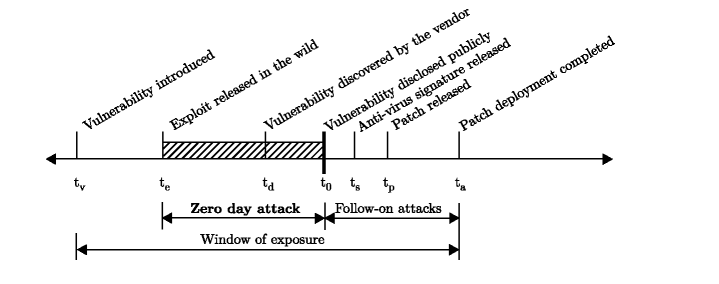
\includegraphics[width=0.9\textwidth]{background/XYZ1.png}
\caption{Timeline of DNS Abuse Attacks on XYZ Corporation}
\label{fig:figureOne}
\end{figure}

The relationship between this correlation raises questions about the attackers' understanding of the inner workings of the firm, as well as insider threats. A closer analysis of the DNS abuse types employed by such offenders revealed that domain hijacking was common \cite{bayer2022study}. Figure \ref{fig:figureTwo} shows how various DNS abuse techniques were used in the case of XYZ Corporation, and domain hijacking was significantly higher than all other combined methods.
\captionsetup{font= footnotesize}
\begin{figure}[ht!]
\centering
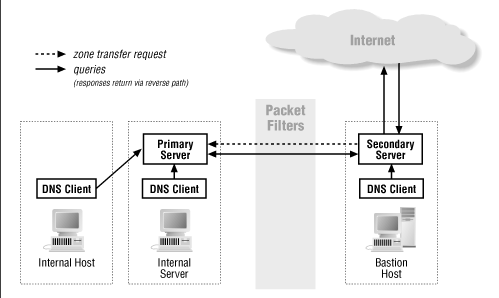
\includegraphics[width=0.8\textwidth]{background/XYZ2.png}
\caption{Distribution of DNS Abuse Techniques Against XYZ Corporation}
\label{fig:figureTwo}
\end{figure}



There is a domain hijacking technique where attackers may effectively take control over a company without authorisation; domain hijacking is one of the major threats to the organisations that are affected. The figure shows that strong security is key to preventing unauthorised access to domain registration accounts; favouring multifactor authentication is the way to keep these attacks away \cite{paz2020cyber}. This case study sheds light on the subtleties of DNS abuse as it targeted XYZ Corporation, showing the importance of understanding and dealing with an unpredictable cyber threat environment. Figures, graphs, and graphs serve to illustrate safeguard attack procedures and give credence to the notion that an all-encompassing cybersecurity strategy is integral to mitigating DNS abuse in the digital landscape of the networked world of our day.

\item\textbf{ Case Study 2: The Sodu.org DDoS Attack }

The "sodu.org" domain was a target of one of the most serious DNS-based Denial of Service (DoS) attacks of September 2012 that affected the DNS infrastructure around the globe Cisco's Security Intelligence Operations (SIO) indicated that the attack was discovered through anomalies of traffic spikes seen across sensors in the Eastern United States, Western United States, and Central Europe \cite{ Middleton2024}. It received over 10 billion query requests in total, nearly 695 gigabytes of traffic. These requests are the A record queries sent to org Generic Top-Level Domain (gTLD) nameservers. The attack, which went on to be repeated over two days of the conference, in a first incidence lasting about 5.5 hours and about 5 hours in a subsequent occurrence, exploited vulnerabilities in DNS infrastructure to drown servers in spoofed requests, causing huge gTLD traffic spikes and showcasing the potential that DNS-based DoS attacks have to derail Internet functionality.

\captionsetup{font= footnotesize}
\begin{figure}[ht!]
    \centering
    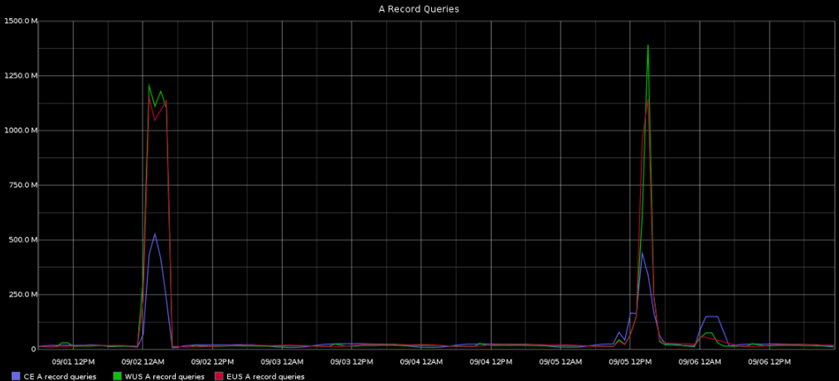
\includegraphics[width=0.8\textwidth]{background/DNSTRaffic.png}
    \caption{DNS A Record Traffic of the Sodu.org DDoS Attack }
    \label{fig:figureSeven}
\end{figure}

\captionsetup{font= footnotesize}
\begin{figure}[ht!]
    \centering
    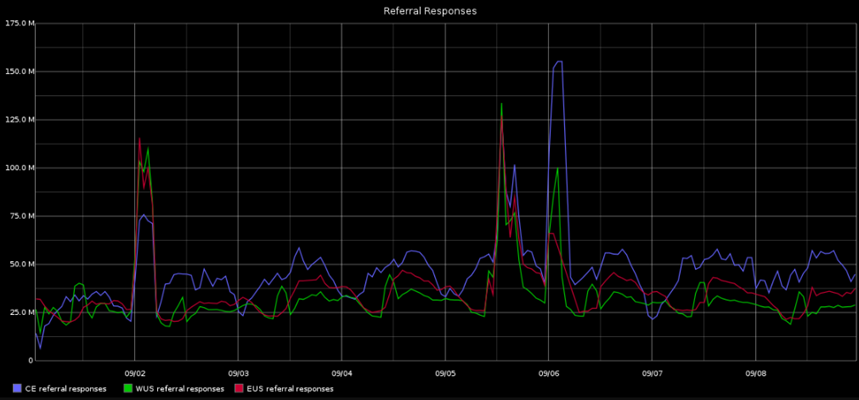
\includegraphics[width=0.8\textwidth]{background/DNSRef.png}
    \caption{ DNS Referral Response Traffic Sodu.org DDoS Attack}
    \label{fig:FigureEight}
\end{figure}

\vspace{200pt}


\item\textbf{ Case Study 3: DNS Amplification Attacks Utilizing DNSSEC }

The DNS amplification attack is one form of DNS abuse that has been prominent more prominently seen in October 2012. This uses the DNSSEC protocol and uses the very nature of the DNSSEC protocol whereby it can store large EDNS0 buffer sizes that it is able to produce huge quantities of traffic heading towards IP addresses totally swamping the links and dramatically reducing the amount of legitimate traffic exchanges possible \cite{ Middleton2024}.  The second big incidence of observation by Cisco SIO was millions of ANY response queries, which were sent to specific IPs, and the quantity clearly passed the normal DNS traffic. These are quite interesting attacks as they leverage the DNS query type 'ANY' and abuse of open recursive resolvers to have more effects. DNSSEC and EDNS0 are additional mechanisms given for the sake of increasing the security of DNS; however, the use of these mechanisms enables attackers to increase the severity of their attack.

\captionsetup{font= footnotesize}
\begin{figure}[ht!]
    \centering
    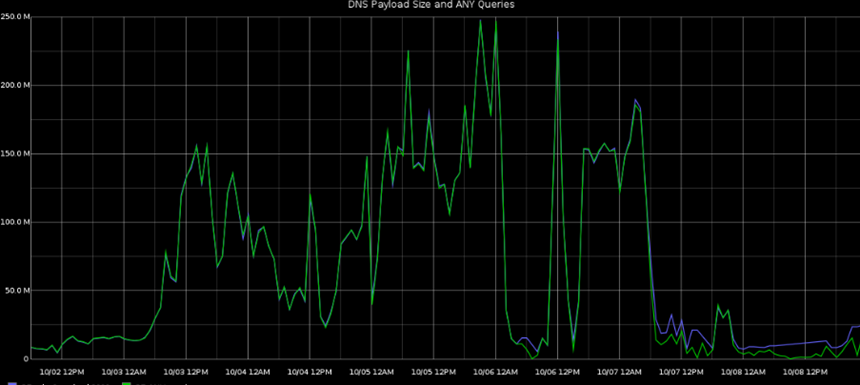
\includegraphics[width=0.9\textwidth]{background/UDP.png}
    \caption{UDP "ANY" Packet Counts and EDNS 9000 Payload Size Counts}
    \label{fig:figNine}
\end{figure}

\item\textbf{ Case Study 4: OilRig DNS Tunneling Attack }

The case of OilRig reflects the use of custom DNS Tunneling protocols for command and control (C2) operations, thus making it dual use in nature, both in normal operation and on a fallback communication channel \cite{paloaltonetworks2021dnsattacks}.The xHunt campaign followed a similar trend of including Snugy backdoor implants in Middle Eastern government organization targets and keeping track of them using DNS tunneling for communication with its C2.  Which are examples that underscore the strategic use by adversaries of DNS tunneling techniques for stealthiness and resilience within the context of their operations. 

\captionsetup{font= footnotesize}
\begin{figure}[ht!]
    \centering
    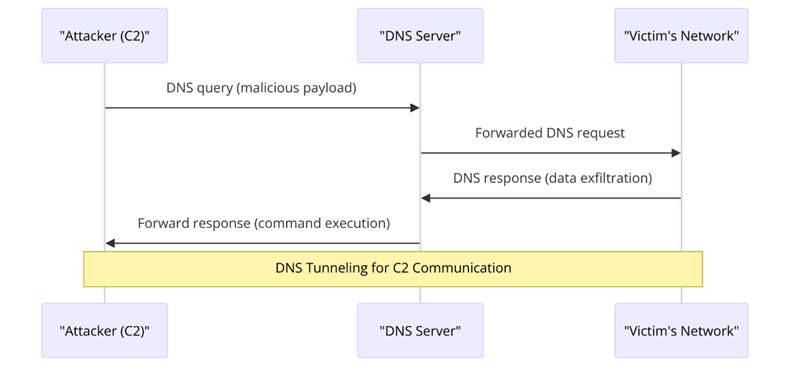
\includegraphics[width=0.9\linewidth]{background/DNSTuu.png}
    \caption{DNS tunneling communication between the attacker's command and control (C2) infrastructure and the victim's network}
    \label{fig:figTen}
\end{figure}
\vspace{100pt}


\item\textbf{ Case Study 5:  SUNBURST Utilization of DGAs}

SUNBURST backdoor associated with the breach of the SolarWinds supply chain represents a case in which the use of DGAs is critical, if not only, to conceal communications and system details \cite{paloaltonetworks2021dnsattacks}. "The SUNBURST backdoor applies deep use of DNS manipulation for evasion purposes and subsequent attack stages through encoding basic system identifiers and usage of DGAs for C2 check-ins.

\captionsetup{font= footnotesize}
\begin{figure}[ht!] 
    \centering
    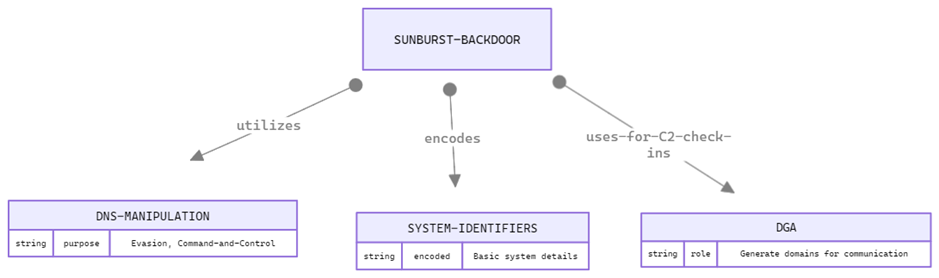
\includegraphics[width=0.9\linewidth]{background/SUNDNS.png}
    \caption{SUNBURST backdoor's utilization of DGAs and its associated components}
    \label{fig:figEleven}
\end{figure}

\vspace{40pt}



\item\textbf{ Case Study 6: Fast Flux Techniques}
The presence of several C2 domains related to the Smoke Loader malware family using Fast Flux techniques only further underscores the difficulties associated with the tracking and eradication of DNS-enabled threats. \cite{paloaltonetworks2021dnsattacks}.The major takeaway in the rapid rotation of IP addresses of this method points to the dynamism of strategies used in communications by malware, thus improving the means of defence by cybersecurity.

\captionsetup{font= footnotesize}
\begin{figure}[ht!]
    \centering
    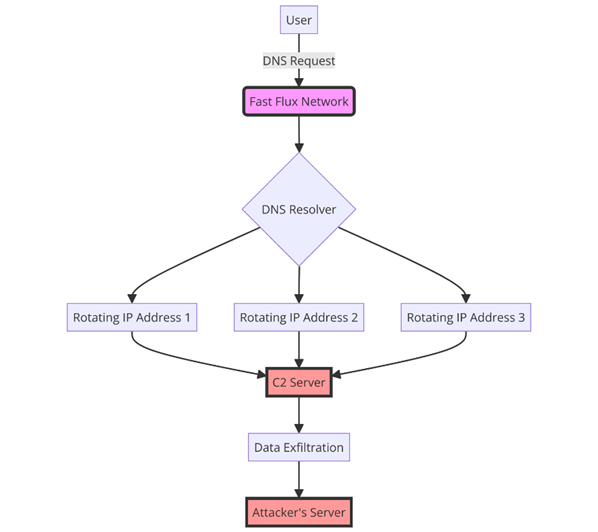
\includegraphics[width=0.7\linewidth]{background/FastFluDNS.png}
    \caption{The usage of Fast Flux techniques by the Smoke Loader malware family for dynamic C2 domain communications}
    \label{fig:figTweleve}
\end{figure}
\vspace{120pt}

\item\textbf{Case Study 7:  Malicious Newly Registered Domains (NRDs)}

The malicious NRDs opportunistically crafted in the milieu of the pandemic expose how threat actors leverage current events for engineering targeted attacks. From domains that mirror COVID-19 information resources to those faking government relief programmes, the evolution of such attacks reflects a calculated approach to exploiting public interest and vulnerabilities. \cite{paloaltonetworks2021dnsattacks}

\captionsetup{font= footnotesize}
\begin{figure}[ht!]
    \centering
    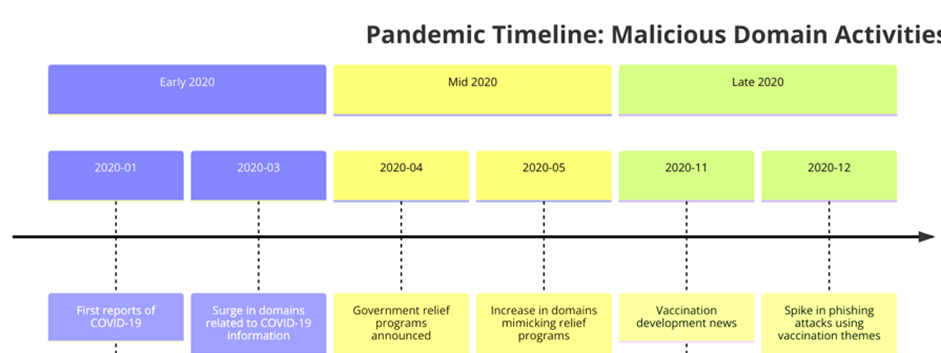
\includegraphics[width=0.9\linewidth]{background/PandemicTime.png}
    \caption{The usage of Fast Flux techniques by the Smoke Loader malware family for dynamic C2 domain communications.}
    \label{fig:figThirteen}
\end{figure}

\end{enumerate}





\section{Challenges and Future Directions}

Mitigating DNS abuse demands an immediate stop to the escalation and rapid evolution of cyber threats, underscoring the critical need for swift global cooperation and the implementation of advanced technology. The key challenge is to achieve a fine balance between reducing false positives and accurately identifying genuine threats, while simultaneously advancing beyond the limitations of outdated technologies. \cite{pour2023comprehensive} The future of this domain largely depends on researchers' ability to enhance technological solutions, particularly focusing on the improvement of AI algorithms for deeper analysis of DNS traffic patterns. This opens a promising pathway for the creation and application of locally developed tools, providing innovative strategies to strengthen DNS defences. The ability to navigate the complex landscape of DNS abuse will require stakeholders to be agile in responding to emerging threats and developing novel solutions. The collective push towards the evolution of technology and methodologies will play a pivotal role in shaping effective DNS abuse management strategies in the years ahead.


\subsection{Identification of Current Challenges}

Mitigating DNS abuse involves developing strategies that should be not only proactive but kept constantly up to date to handle the changing environment of cyber threats. The fluid nature of these threats means updating current protocols as well as developing new defence methods. With cybercriminals constantly revising their methods of capitalizing on the vulnerability of DNS, it has become imperative for the cybersecurity industry to continuously update its defence mechanisms \cite{bhattacharya2023dns}. Being a global phenomenon, the internet, and hence DNS abuse being transnational in character, there is no other alternative than international cooperation. The effectiveness of the DNS abuse management would be based on collaborative work across national borders, where experts in different geographical areas come together to share their knowledge and resources \cite{altulaihan2022cybersecurity}. Legal and regulatory framework varies in the several jurisdictions, thereby making it difficult to reach a consensus on the regulations, standards, and enforcement action. Another big challenge is that, to mitigate DNS abuse, the requirement for driving down both false positives and negatives is necessary. Balance must be established in such a way that rather strict measures may reduce user experience, while, at the same time, being liberal might bring less detection of malicious activities \cite{lyu2022survey}. The cybersecurity community must continue to advance its detection and response capabilities, due to the increasing levels of sophistication used by DNS abusers. This will keep the security and integrity of the DNS system in good shape, hence protecting this vital part of internet infrastructure.

\subsection{Discussion on Future Research Directions and Technologies}

When planning to mitigate the DNS abuse in the future, discussing new research ideas and upcoming technology is crucial. The constantly changing state of Internet threats requires us to continually create new things. This is so people can stay one step ahead of the bad people. Future work on DNS abuse needs to start by building better tools. These can help to address how bad guys on the Internet keep changing their tricks \cite{bovenzi2023blockchain}. This means that we need to look at more complex AI and machine learning tools that can understand the details of web traffic. This will make the results more accurate and stop wrong signals from being sent. Moreover, there is a rising need to use blockchain tech to make domain registration safer and stop any bad or harmful changes, as it provides decentralised domain name resolution unlike traditional DNS systems, which rely on a central authority to resolve domain names, a Blockchain DNS operates on a network of distributed nodes in which each node has a copy of the entire blockchain ledger, so it can independently verify and resolve domain name requests, which not only makes the system more resilient to attacks but also prevents censorship and control by a single entity. \cite{FinanceStrategists2023BlockchainDNS}.  People should have easy methods to report DNS abuse. This will make sure everyone knows about dangers \cite{gu2021iot}. Working together in the world is very important because computer dangers go beyond borders. So everyone in the world needs to work together. 


\section{Conclusion}

DNS abuse continues to be a big issue. Present plans, while sometimes useful, require constant adjustment and getting better. It's key to have solutions for fixing issues available. This helps to build trust and work well with those involved. Abusing DNS in new ways brings fresh issues that require clever solutions. AI and machine learning can help find things, but we need to show how they work better so that people can keep bad people under control. Learning from real-life situations teaches us a lot about good and bad ways of being open. This helps us create the best methods for our business. There are still issues with showing and stopping DNS abuse while trying to find new ways to mitigate this DNS abuse. People need to continue learning and working as a team. People should focus on better technology, joining forces with other nations, and using common methods of sharing information in the future. As the internet changes, we must stay active and work together to stay ahead of bad people who want to hurt us. 

\section{Summary of Findings}

The study on DNS abuse looked at current ways, checked new trends, talked about tech advancements, and explored real examples in life. The search for ways in the plans to mitigate DNS abuse showed the value of clear communication and honesty in building trust with the community. People are finding new ways to abuse the DNS system. Researchers have to keep making new things, so they don't get caught by changing dangers. Improvements in technology, especially with artificial intelligence and learning machines, showed how automation can make it easier to spot dangers. But it also made things harder to understand, and this needs careful attention. Examples from real life showed what did and did not work in making DNS abuse clearer. These provided essential advice for the business. Issues with making things clear and stopping wrong actions were found. This shows how important it is to continue learning and working with others. In the future, discussing issues and future plans will show the need for creative studies, help from other nations, and common ways to share information. 



\section{Figures}
Graphs, pictures and other images should be included in your report as a numbered, captioned figure. An example is given in Figure \ref{veldis}.

%%%%%%%%%%%%%%%%%%%%%%%%%%%%%%%%%%%%%%%%
\begin{figure}[h]
      \centering
      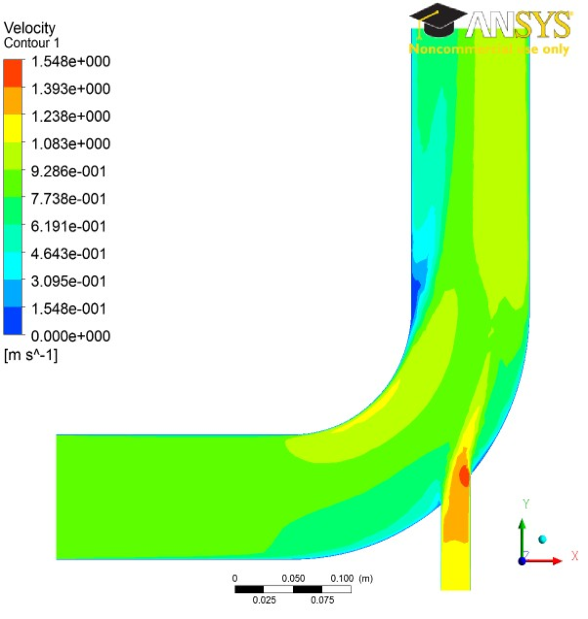
\includegraphics{background/5e1-1.pdf}
      \caption{Velocity distribution on the mid-plane for an inlet velocity for case 1.}
      \label{veldis}
\end{figure}
%%%%%%%%%%%%%%%%%%%%%%%%%%%%%%%%%%%%%%%%

The figure and caption should be centred. The figure numbering starts at 1 at the beginning of each chapter. The caption should provide a brief description of what is being shown. The figure should appear in the document after it is referred to in the text. No figure should be included which is not referred to in the text. Ensure that the size and resolution of images imported from software are sufficient to read any text.

\section{Tables}
Tables are an important way of displaying your results. Table \ref{tab:treatments} is a sample table, adapted from the Master/Doctoral Thesis template at \url{http://www.latextemplates.com/cat/theses}, which was generated with this code:

{\footnotesize
\begin{verbatim}
\begin{table}[b]
\caption{The effects of treatments X and Y on the four groups studied.}
\label{tab:treatments}
\centering
\begin{tabular}{l l l}
\toprule
\textbf{Groups} & \textbf{Treatment X} & \textbf{Treatment Y} \\\midrule
1 & 0.2 & 0.8\\
2 & 0.17 & 0.7\\
3 & 0.24 & 0.75\\
4 & 0.68 & 0.3\\
\bottomrule\\
\end{tabular}
\end{table}
\end{verbatim}
}

\begin{table}[b]
\caption{The effects of treatments X and Y on the four groups studied.}
\label{tab:treatments}
\centering
\begin{tabular}{l l l}
\toprule
\textbf{Groups} & \textbf{Treatment X} & \textbf{Treatment Y} \\
\midrule
1 & 0.2 & 0.8\\
2 & 0.17 & 0.7\\
3 & 0.24 & 0.75\\
4 & 0.68 & 0.3\\
\bottomrule\\
\end{tabular}
\end{table}

Tables are numbered in the same way as figures. Typically tables also have a short caption, but this is not universally true. The number and caption appear above the table, not below as with figures. Again, no table should appear in the report which has not been referred to in the text. Tables should come after they are discussed in the text. The exact formatting of the table depends somewhat on the content of the table, but in general, the text in the table should be the same font and size as the main text. 

\section{Equations}
All equations should be numbered sequentially. The numbering restarts automatically at the beginning of each chapter, and contains the number of the chapter alongside the equation number. Unlike figures and tables, you may not need to refer to every equation in the text. You should take care to format equations properly. Do no simply try to use plain text. Use the equation layout facilities. An example of how equations should appear is shown in \eqref{sampleequation}. Here is the code for it:

{\footnotesize
\begin{verbatim}
\begin{equation}
\textrm{div}(\underline{u}) = \frac{\delta u}{\delta x} + \frac{\delta v}{\delta y} +
        \frac{\delta w}{\delta z} = 0
\label{sampleequation}
\end{equation} 
\end{verbatim}
}

\begin{equation}
\textrm{div}(\underline{u}) = \frac{\delta u}{\delta x} + \frac{\delta v}{\delta y} + \frac{\delta w}{\delta z} = 0
\label{sampleequation}
\end{equation} 

\section{Referencing published work}
It is important to give appropriate credit to other people for the work that they have shared through publications. In fact, you must sign a declaration in your report stating that you understand the nature of plagiarism. As well as avoiding plagiarism, citing results or data from the literature can strengthen your argument, provide a favourable comparison for your results, or even demonstrate how superior your work is.

There are many styles to reference published work. For example, the parenthetical style (which is also called the \emph{Harvard style}) uses the author and date of publication (e.g. ``Smith and Jones, 2001''). There is also the Vancouver style (or the \emph{citation sequence style}). In the IEEE style, which is used in this document in the default setup, the publications are cited using bracketed numbers which refer to the list in the References section at the end of the report. The references are listed in the order that they are cited in the report. A variant is \emph{name sequence style}, in which the publications are referenced by number, but the list is arranged alphabetically. The following paragraph shows the use of the IEEE style: 

\begin{quote}
Several studies have examined the sound field around tandem cylinders generated by flow\cite{fitzpatrick2003flow,finnegan2010experimental}, while other investigations have focused on the effect of an applied sound field on the flow\cite{hall2003vortex}. Papers from conference proceedings\cite{jordan2001array}, books\cite{paidoussis2010fluid} and technical reports\cite{reyes2007power} can be dealt with in the same style.
\end{quote}

The IEEE style has the advantage that it is a little more compact in the text and does not distract from the flow of the sentence if there are a lot of citations. However, it has the disadvantage that it is not immediately clear to the reader what particular work has been referenced. You can use author names directly and discuss the work of Finnegan et al. \cite{finnegan2010experimental} similar to this sentence to make it more readable. 

It actually does not matter which particular referencing style is used as long as three important considerations are observed:
\begin{itemize}
\item the referencing style used throughout the document is consistent;
\item all material used or discussed in the text is properly cited;
\item nothing is included in the reference list that has not been cited.
\end{itemize}

Check with your supervisor as they may have a strong opinion on what you should use

This template has a suitable referencing style already set up -- you should use it and use the built-in BibTeX system to manage your references. See above for examples of how to cite a reference and look in the \texttt{sample.bib} file to see BibTeX references. It is strongly recommended that you use a bibliographic tool, such as EndNote (check out https://www.tcd.ie/library/support/endnote/), as this will facilitate compliance with these three requirements. Endnote can help you build you .bib file. Remember \href{http://scholar.google.com}{Google Scholar} and other search engines will give you BibTeX references for lots of academic publications. Be aware that Web of Science is more reliable for giving the full record for the BibTeX entry. Otherwise, you can easily make up your own based on the examples in that file.